\newpage
\section {User Experience}
\label{sec:user}

  For service endpoints which run computations in real time, the maintainer of a system might want to understand the endpoint performance on a per-user basis, especially for situations where the system response time is a function of some individual user load\footnote{E.g. in GMail some users have two emails while other have twenty thousand and this induces different response times for different users}.

  To enable this, the \tool must be configured with a way of associating an API call with a given user. There are multiple ways, the simplest of which utilizes again the common expectations of Flask applications that offers a global \code{request} object which contains a \code{session} object which encapsulates information: 

  %\begin{lstlisting}[float,caption=Simply define a custom app-specific function for user retrieval and pass it to the \tool to group information by user,style=custompython]
  \begin{lstlisting}[style=custompython]  
    # app specific way of extracting the user
    # from a flask request object    
    def get_user_id(request):
      sid = int(request.args['session'])
      session = User.find_for_session(sid)
      return user_id

    # attaching the get_user_id function
    dashboard.config.get_group_by = get_user_id

  \end{lstlisting}

  In the Zeeguu case study, one of the slowest endpoints, and one with the highest variability as shown in \Fref{fig:ep} is \epFeedItems: it retrieves a list of recommended articles for a given user. However, since a user can be subscribed to anything from one to three dozen article sources, and since the computation of the difficulty is personalized and it is slow, the variability in time among users is likely to be very large. 


  Figure \ref{fig:tpu} shows some of the results of calling the \epFeedItems endpoint for various users. The figure shows that the response times for this endpoint can vary considerably for different users. 

  \begin{figure}[!ht]
    \centering
    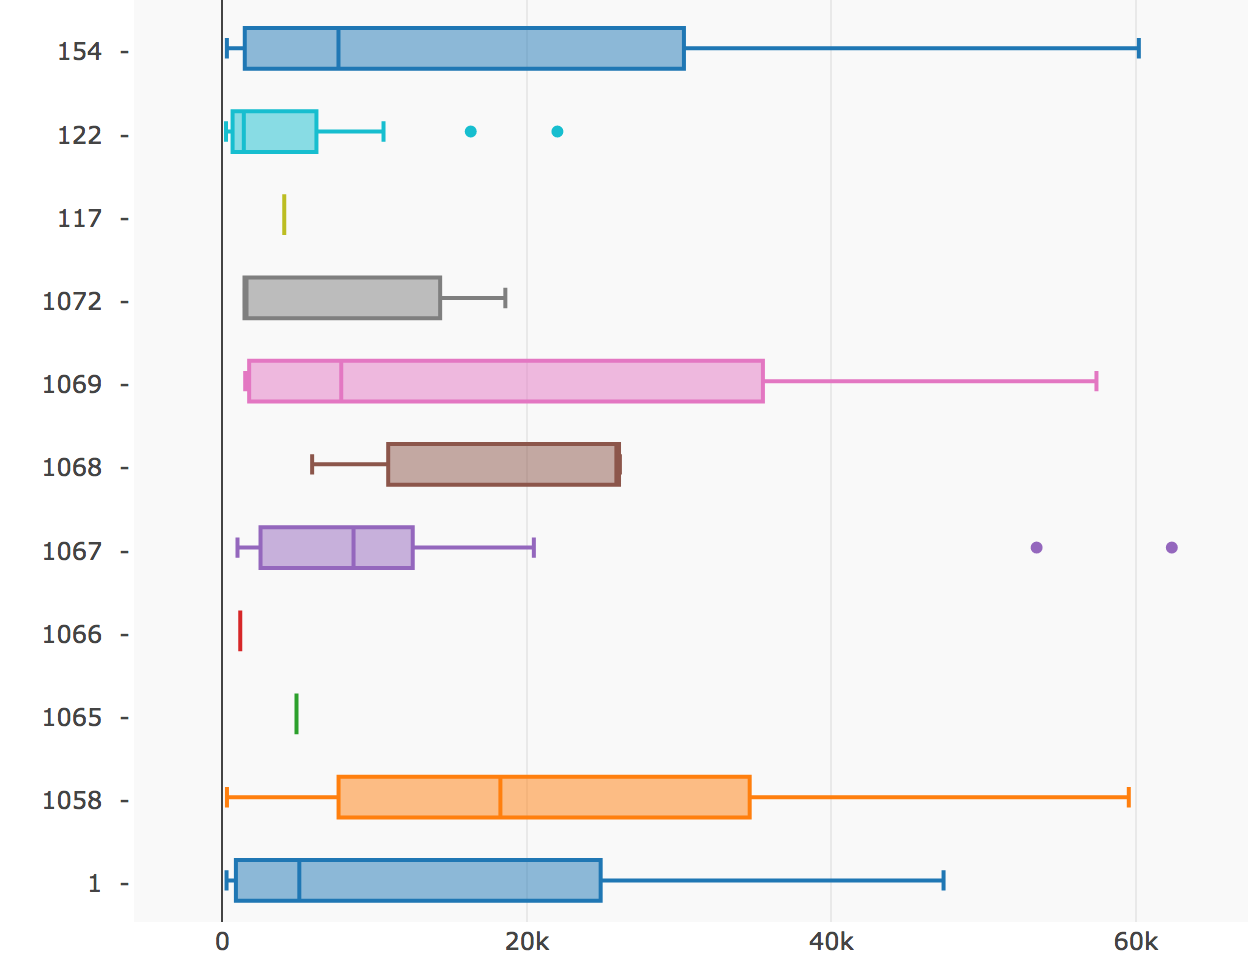
\includegraphics[width=\linewidth]{time_per_user}
    \caption{The \epFeedItems shows a very high variability across users}
    \label{fig:tpu}
  \end{figure}

  \newpage
  \niceseparator

  The limitation of the previous view is that it does not present the information also on a per version basis. To address this, a different visual perspective entitled \perspective{Endpoint Evolving per-User Performance} can be defined. Figure \ref{fig:tuv} presents such a perspective by mapping the average execution time for a given user (lines) and given version (columns) on the area of the corresponding circle. The colors represent users.

  \begin{figure}[!ht]
    \centering
    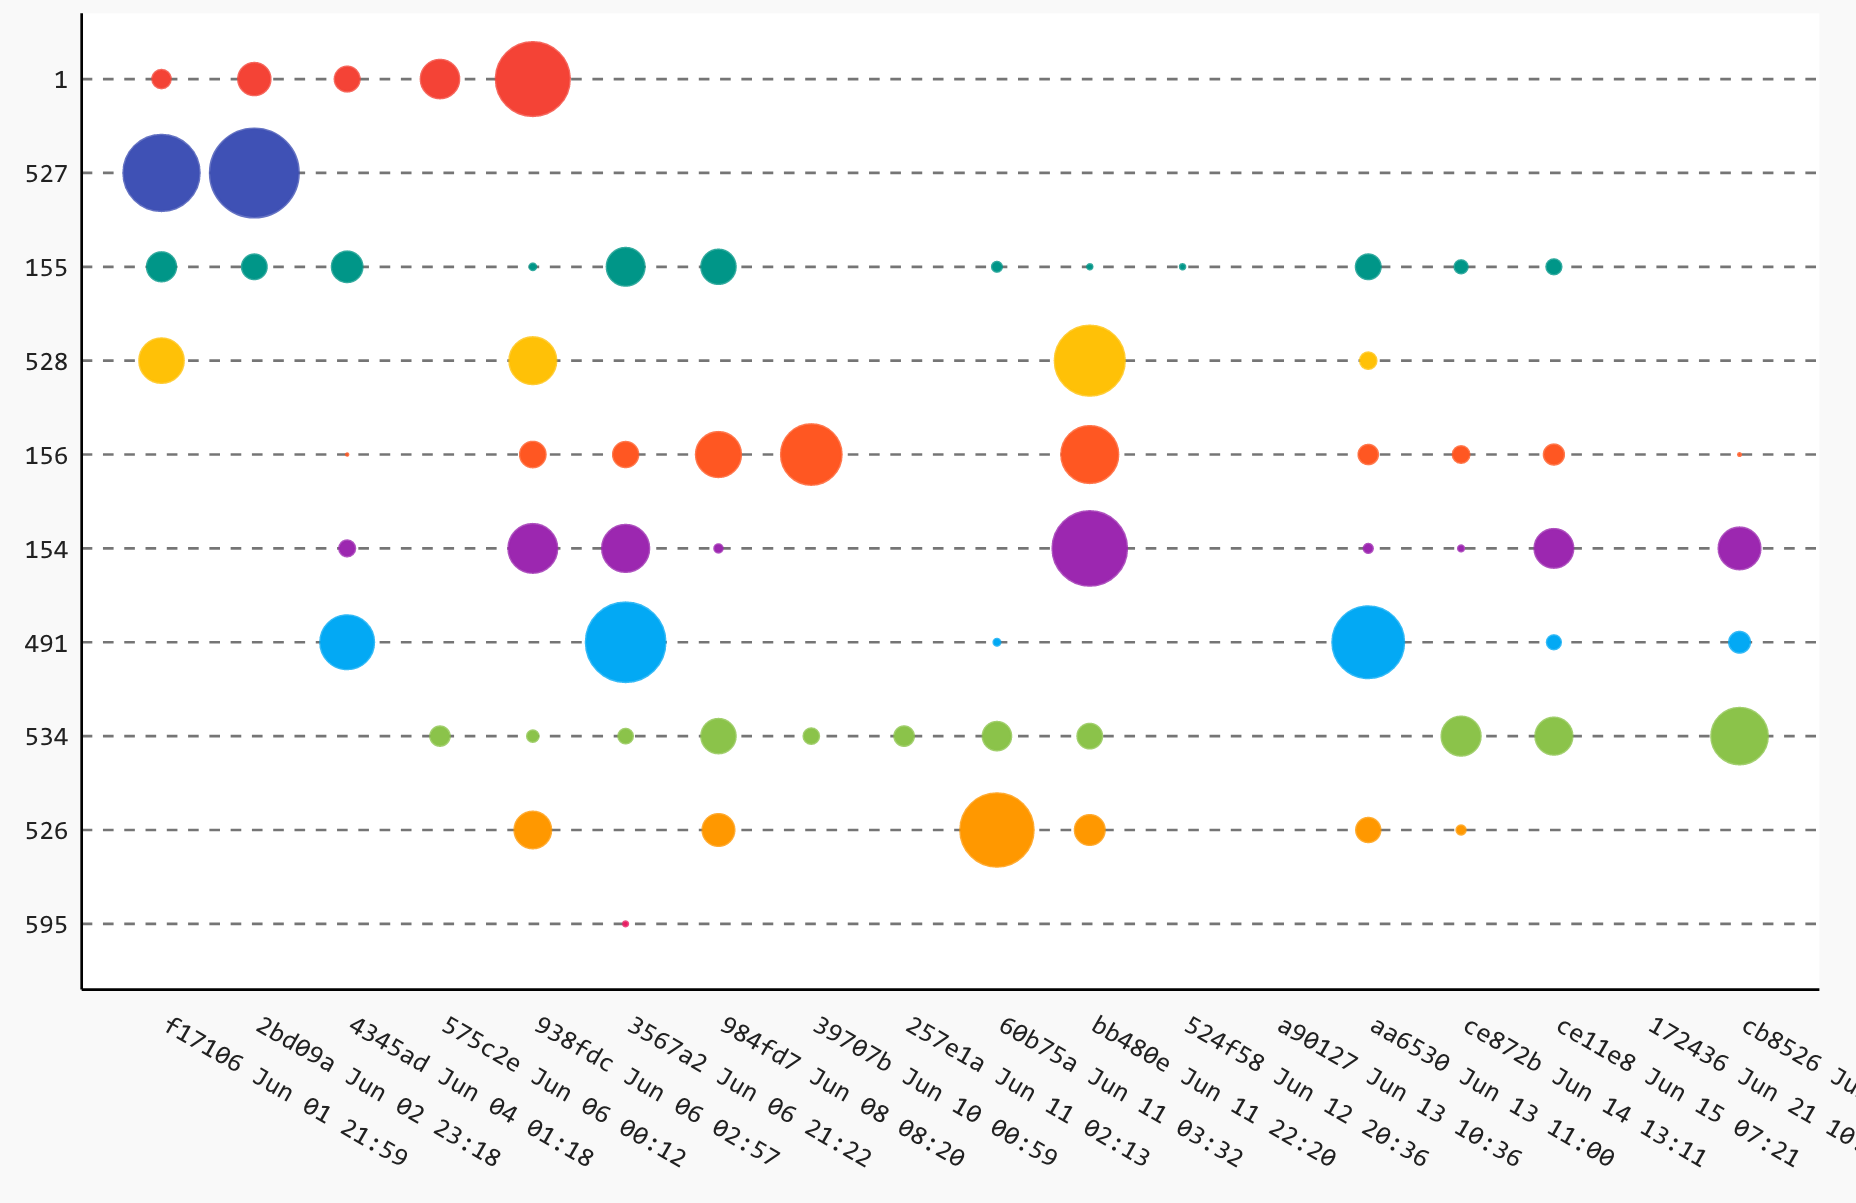
\includegraphics[width=\linewidth]{time_per_user_per_version}
    \caption{This perspective shows that the evolution of response times for individual users (horizontal lines) across versions (the x-axis)}
    \label{fig:tuv}
  \end{figure}

  For the situations in which the user information is not available, the \tool also tracks out of the box information about different IPs. In some cases this might be a sufficiently good approximation of the user diversity and identity. 
  %
  In the interest of space limitations we are not showing this, and quite a few more visualizations provided by the \tool. The interested reader is referred to \Sref{sec:install} for further information on how to install the tool and how to get access to the data of the case study.
